\subsection{Review of common Join Algorithms in Big Data and benefit of Join Ordering for them}
Let's look at common Join algorithm used in two of the most prominent SQL Engines for Big Data: Presto and Apache Spark SQL ~\cite{b13}. We will also see how will reordering help in improving those Join algorithm. Improvements due to Join Reordering has already been reported for these SQL Engines by their implementation of Cost-Based optimization in presence of Statistics ~\cite{b2}, which further strengthens our claim that it is an important Join optimization even in Big Data paradigm.

\subsubsection{Distributed Hash Joins in Presto}

\begin{figure}[ht]
    \centerline{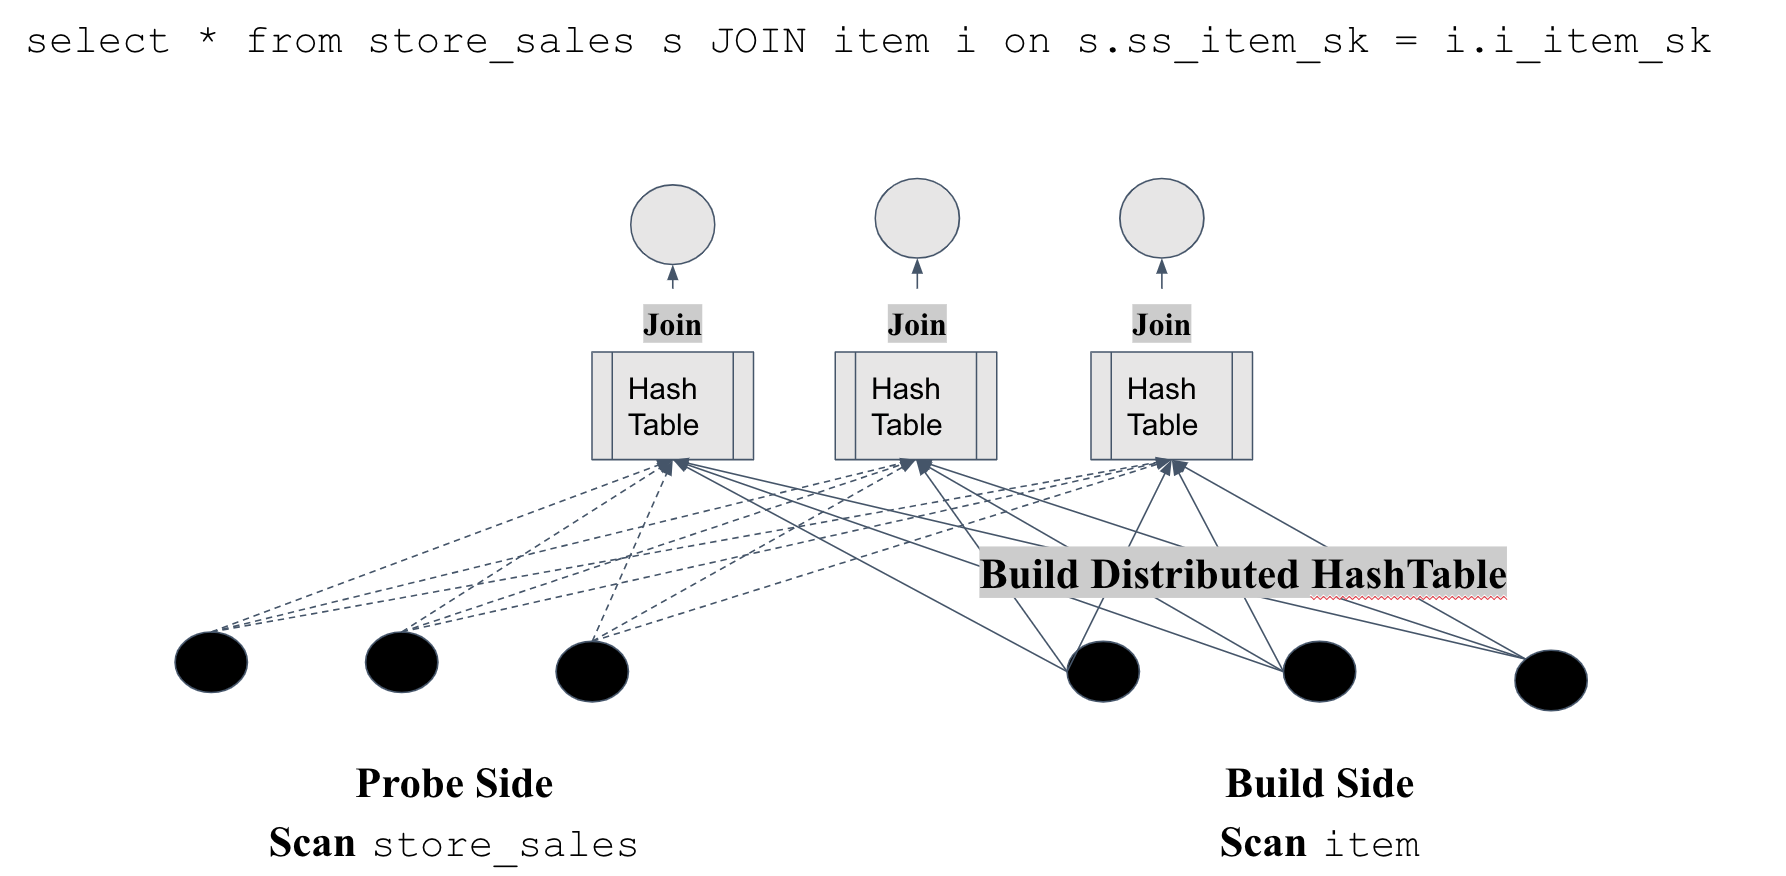
\includegraphics[width=9.5cm]{fig/DistributedHashJoin.png}}
    \caption{Distributed Hash Join}
    \label{distributed_hash_join}
\end{figure}

Distributed Hash Join is most commonly used distributed join algorithm in Presto.
Figure \ref{distributed_hash_join} illustrates this join.
When joining two tables \texttt{store\_sales} and \texttt{item} Presto regards table on the right i.e., \texttt{item} as build side and table on left i.e., \texttt{store\_sales} as probe side.
Build side is used to build distributed hash table. As shown in the figure, after table \texttt{item} is scanned, its rows are hash distributed to different nodes based on join key \texttt{i\_item\_sk}. Once distributed, rows from table B are used to create Hash Table. Rows from the Probe Side are also distributed to different nodes using the same hash on the join key \texttt{i\_item\_sk}. Due to this partitioning \texttt{ss\_item\_sk}  and \texttt{i\_item\_sk} with same values end up in the same node.  Rows of Probe Side once distributed are checked against Hash table to find matching join rows. Here, major cost of the join will be building Hash tables on the Build Side. Hence, join reordering can considerably improve the performance by choosing smaller table as build side whenever possible (like in the cases of INNER Joins).

\subsubsection{Sort Merge Join in Spark}\label{subsubsec:sparkjoin}

\begin{figure}[ht]
    \centerline{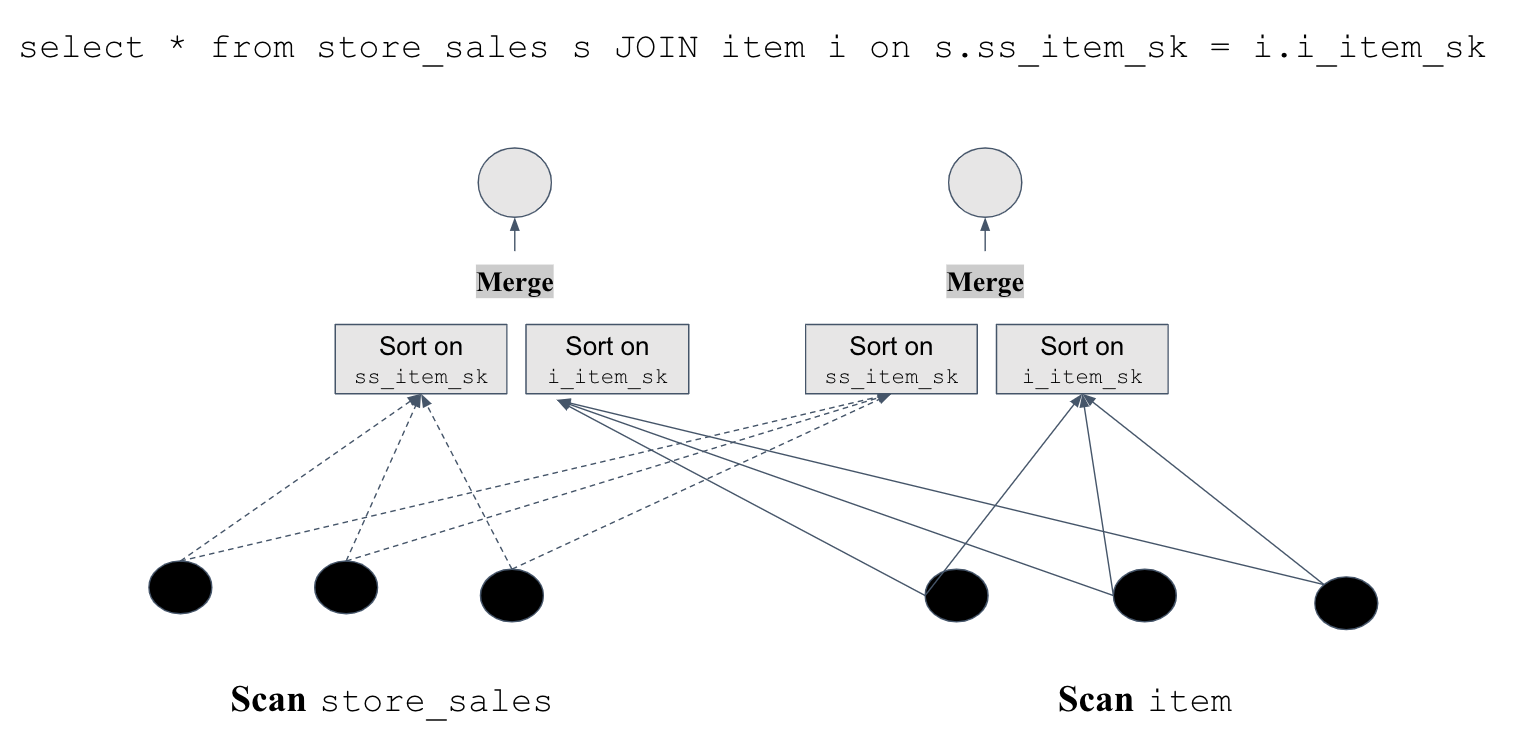
\includegraphics[width=9.5cm]{fig/SortMergeJoin.png}}
    \caption{Sort Merge Join}
    \label{sort_merge_join}
\end{figure}

Spark implements both Sort Merge Join and Hash Join.
Hash Joins are commonly used for Broadcast Joins, where if one of the sides of join is less in size than the threshold set by \texttt{$sql.autoBroadcastJoinThreshold$} then that side's hash table gets broadcasted to nodes with other larger side.
Join is performed locally on those nodes against the broadcasted hash table.

Except for the above case, Sort Merge Join is most commonly used join in Spark. Figure \ref{sort_merge_join} illustrates the Sort Merge Join.
Both tables \texttt{store\_sales} and \texttt{item} are distributed based on hash partitioning on join keys i.e., \texttt{ss\_item\_sk} and \texttt{i\_item\_sk} respectively. Due to this partitioning \texttt{ss\_item\_sk}  and \texttt{i\_item\_sk} with same values end up in the same node. Once rows from each table are distributed, they are individually sorted locally in every node and they are merged together to perform join. Internally Spark while doing merge uses scanner where for every key being considered for merging, one side will be streamed and another side will have rows with merge key buffered. Buffered rows can be spilled to disk too if it crosses memory threshold. In case of INNER Join, left side is streamed and right one will be buffered. So it is better to ensure the buffered side is the smaller one for lesser memory consumption and to avoid spill (spill can affect performance adversely). Hence, Join reordering is essential.

Both the above examples I provided were for a single join. In case of multi-way Join, reordering becomes even more important and can lead to huge performance improvements.